\chapter{Computing K-mer Abundance Histogram}

In this chapter we summarize some of the fastest algorithms for approximating histogram of $k$-mer abundance 
and describe generative probabilistic models used for genome length estimation.

\section{Computing K-mer Abundance Histogram}
\label{sec:algorithms}

The simple approach to compute $k$-mer abundance histogram would be firstly to compute $k$-mer counts --
exact numbers of occurrences of all $k$-mers -- and then count different $k$-mers with $j$ occurrences for each $j$.
Since the role of $k$-mer counts is important in bioinformatics, there exist many tools that
compute $k$-mer counts. In the first subsection we briefly summarize these algorithms.

$k$-mer counting is a computationally demanding task for a large amount of $k$-mers, however.
As we are only interested in the histogram, the problem of $k$-mer counting can be avoided,
allowing us to estimate the histogram very efficiently without an intermediate step.

\subsection{Exact K-mer Abundance Counting}
\label{sec:exact-algorithms}
In the naive hashing algorithm, a hash function $h$ would uniformly distribute strings of length $k$ to a hash table $T$. 
We would store the number of occurrences of a $k$-mer $s$ in the counter $T[h(s)]$. In a single scan through all the reads we
would then increment the appropriate counters. This solution works well for millions of $k$-mers, but as
the number of distinct $k$-mers increases, we must use larger hash tables in order to prevent collisions.
This solution becomes much slower when the hash table $T$ becomes larger than RAM available.

A few techniques were used to decrease the time and memory consumption by a constant factor. 
These improvements allowed the hashing approach to be used in practice:

\begin{itemize}
\item Based on an observation that most of the $k$-mers with only one occurrence come from erroneous reads,
BFCounter \cite{Melsted2011} uses a Bloom filter to exclude rare $k$-mers from hash table thus saving memory.

\item Jellyfish \cite{Marcais2011} software uses a thread-safe hash table utilizing the advantage of parallel computing.

\item To decrease the size of hash table, Disk Streaming of K-mers (DSK) \cite{Rizk2013} algorithm scans the input data in more
iterations, processing only a subset of $k$-mers in each iteration. A second hash function is used to determine the subset
(and the iteration) for each $k$-mer (a similar principle is used to randomly sample $k$-mers in section \ref{sec:simple-sampling}).
\end{itemize}

A different, but still memory-demanding, approach based on suffix arrays was used in Tallymer software \cite{Kurtz2008}.
A suffix array is a data structure holding all suffixes of a string sorted in a lexicographical order. Suffixes with identical
prefixes of length at least $k$ represent different occurrences of a $k$-mer. Since they are stored in a sorted order, 
abundances of $k$-mers can be computed by grouping adjacent suffixes. 

\subsection{Approximating the Histogram}
As we drop the requirement to compute the exact histogram, it is no longer necessary to store the abundance of each $k$-mer.
This provides a way to reduce the amount of required memory from dozens of gigabytes 
to hundreds of megabytes, allowing these computations to be performed on a personal computer rather than on a cluster.  

To use all data available we must, however, still analyse every $k$-mer of every read so the time complexity of the
following algorithms will still be at least linear in the number of $k$-mers.

\subsubsection{Simple sampling from $k$-mers}
\label{sec:simple-sampling}
The simplest optimization, which was used in a tool KmerGenie \cite{Chikhi2013}, is to sample from the $k$-mers.
With the parameter $s$, we can choose a hash function $\rho_s: \{A,C,G,T\}^k \rightarrow \{0, 1, \dots, s-1\}$ 
that uniformly distributes the $k$-mers to $s$ buckets. Afterwards, we can compute the histogram by a naive
hashing approach or by any other algorithm presented in the previous section \ref{sec:exact-algorithms} using only
the $k$-mers that hashed to 0. Of all the distinct $k$-mers, only a randomly selected fraction of $1/s$ is considered.

The authors used value $s=1000$ in their experiments. As it can be seen from the experimental data (fig. \ref{img:kmergenie-sampling-accuracy}),
the approximation closely follows the exact histogram $f$ at abundances with higher values of $f_i$ -- if enough of unique $k$-mers of abundance 
$i$ were sampled. Fewer $k$-mers reach higher abundances $i$ and thus even fewer of them are sampled, which leads  
to decreased relative precision of approximation of lower values $f_i$. The authors did not include any analytical bounds of errors, however.

\begin{figure}
\centerline{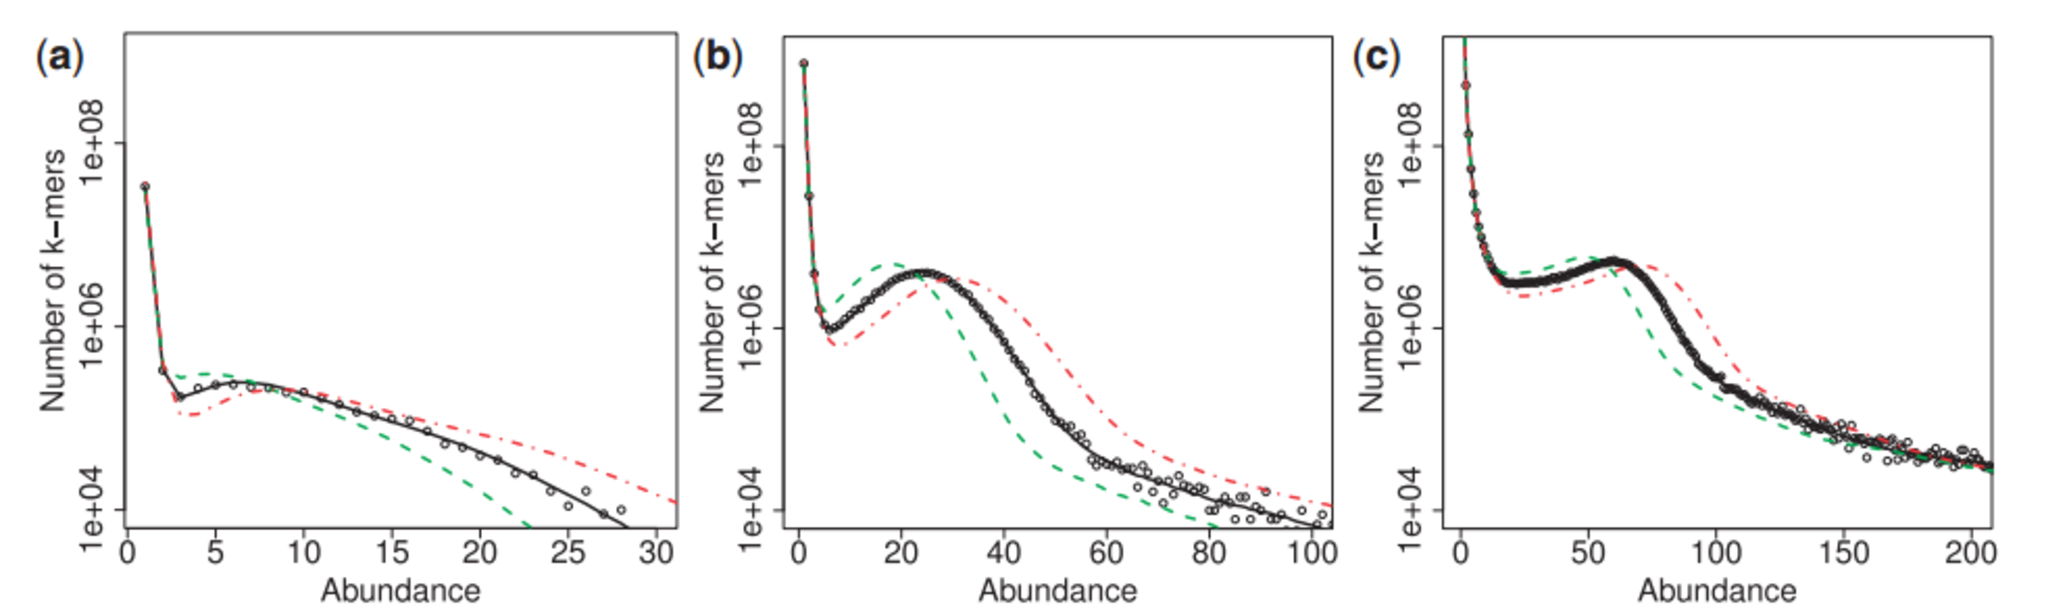
\includegraphics[width=1.1\textwidth]{images/kmergenie-sampling-accuracy.pdf}}
\caption[Accuracy of KmerGenie Sampling]{The accuracy of the sampling method. Reprinted from the original paper \cite{Chikhi2013}. 
The panels reflect the three datasets. Each plot shows the exact
histogram curves for $k=51$ (solid black curve), $k=41$ (dash-dot red curve) and $k=61$ (dashed green curve). The approximate (sampled) histogram is
shown using black dots. Note that $f_i$ is shown on a log-scale, exaggerating the differences at lower $f_i$ values.}
\label{img:kmergenie-sampling-accuracy}
\end{figure}

\subsubsection{Multilevel sampling}
The inspiration for the next approach comes from streaming algorithms.
Streaming algorithms are used to process a sequence of items (in our context $k$-mers) usually 
in only one pass with limited memory and time usage per item. These algorithms often maintain
an approximate summary or a sketch of the previously viewed items. The common problem solved by
streaming algorithms is counting distinct elements in a stream \cite{WikiStreamingAlg}.

In 2014 Melsted and Halldórsson introduced a streaming algorithm KmerStream \cite{Melsted2014}
which was able to estimate the number of distinct $k$-mers ($F_0 = \sum_{i=1}^{m} f_i$) and also
the number of $k$-mers with abundance one ($f_1$) -- $k$-mers with only one occurence.

This algorithm was further improved by Sivadasan et al.\ in 2016 \cite{Sivadasan2016} and their software 
Kmerlight was able to estimate the whole histogram ($f_1, f_2, \dots , f_m$).

\medskip
Firstly, Kmerlight processes a stream of $k$-mers and updates the sketch with each $k$-mer.
The estimates of $F_0$ and $f_i$ are computed from the content of the sketch in the end. 

Kmerlight's sketch consists of $W=64$ levels. There is a hash table $T_w$ at level $w$ with $r$ counters -- $T_w[0], T_w[1], \dots, T_w[r-1]$.
Each counter $c$ stores its value $T_w[c].v$ (number of elements stored in the counter) and an auxiliary information $T_w[c].p$ from range
$0, \dots, u-1$.


\paragraph{Update}
\begin{itemize}
\item For a distinct $k$-mer, its level is selected so that the probablity that level $w$ is selected is $1/2^w$. The $k$-mer is hashed
into a random integer of $W$ bits and the number of trailing zeroes determines the level $w$, thus all occurences of the same
$k$-mer will be placed to the same level $w$.

\item Next, using a different hash function $h: \{A, C, G, T\}^k \rightarrow \{ 0, \dots, r-1\} \times \{ 0, \dots, u-1\}$, the $k$-mer is uniformly hashed 
into a pair $(c, j)$. 
\begin{itemize}
\item If the counter $c$ at level $w$ is empty, its value is increased to 1 and $j$ is stored as an auxiliary information.
\item If the counter $T_w[c]$ is not empty, but the auxiliary information in $T_w[c].p$ is equal to $j$, the counter value $T_w[c].v$ is increased.
\item Finally, if $T_w[c].p \neq j$, the counter is marked as dirty with value -1.
\end{itemize}
\end{itemize}
All occurences of the same $k$-mer will be stored in the same counter, and the value of the counter should correspond to the abundance of this $k$-mer.
Since two or more different $k$-mers may hash into the same counter at the same level $T_w[c]$, collisions may occur. The auxiliary information
helps to detect these collisions.


\paragraph{Estimator of $F_0$}
Since $F_0 / 2^w$ distinct $k$-mers are hashed into the level $w$, the probabilty, that a counter at level $w$ remains empty
is $p = (1 - \frac{1}{r})^{F_0/2^w}$. The expected number of empty counters at level $w$ is thus $r \cdot p$. Let us denote the
number of observed empty counters as $t_0$. Using $t_0$ and the previous equations, we can easily derive the estimator of $F_0$:

$$ \hat F_0 = 2^w \cdot \frac{\ln(t_0/r)}{\ln\left(1 - \frac{1}{r}\right)} $$

To estimate the number of distinct $k$-mers, we choose one level of the sketch $w^*$, so that half of counters of $T_{w^*}$ are empty
-- the number of empty counters at this level is closest to $r/2$. In \cite{Melsted2014} it has been shown that selecting this level
provides bounded error of $\hat F_0$ with guaranteed probability.

\paragraph{Estimator of $f_i$}
The expected number of distinct $k$-mers with abundance $i$ hashed to the level $w$ is $f_i / 2^w$.
When a $k$-mer is hashed into the level $w$, the probabilty, that it is stored in a collision-free counter
is $(1 - \frac{1}{r})^{F_0/2^w - 1}$, which is probability, that no other $k$-mer from level $w$ will get hashed into the same counter.
Thus we can estimate the number of collision-free counters with value $i$ as  $f_i / 2^w \cdot (1 - \frac{1}{r})^{F_0/2^w - 1}$.
If we denote the number of observed collision-free counters with value $i$ as $t_i$, we can derive the estimator of $f_i$:

$$ \hat f_i = t_i \cdot 2^w \cdot \left(1 - \frac{1}{r}\right)^{1 - F_0/2^w} $$

Again, one level $w^*$ is selected to estimate $f_i$, so that it maximizes $t_i$ -- the number of collision-free counters with value $i$.
This decision was not discussed by the authors, but it seems to be a reasonable choice, since higher levels would contain much
less counters with value $i$ and lower levels would countain much less collision-free counters.

The collision detection is unable to detect all collisions, however. The value $t_i$ is based on the non dirty counters, 
but these include both true positives (collision-free counters) and false positives (counters with undetected collision).
The authors have shown that the expected number of false positive at one level is $r/u$ \cite{Sivadasan2016} and that 
parameter $u$ can be set to make false positives negligible.

\medskip

To further decrease the variance of estimates and to make use of multiprocessing, $t$ instances of sketch are run concurrently.
Estimate $\hat F_0$ is then selected as median of $\hat F_0^{(1)}, \dots, \hat F_0^{(t)}$, and also estimates of $f_i$ are
selected as medians from $t$ instances. 

\paragraph{Accuracy and complexity}
The parameters $r$, $u$ ant $t$ can be altered to achieve a viable memory-accuracy trade-off.
The algorithm uses $O(t \cdot r \cdot \log(F_0))$ memory words by $t$ instances of sketches with $\log F_0$ levels with $r$ counters each,
and an update of $t$ sketches (processing of one $k$-mer) demands $O(t)$ time.

The authors have shown that the algorithm computes estimates $\hat F_0$ and $\hat f_i$ for sufficiently large $f_i$ ($f_i \geq F_0 / \lambda$)
with a bounded relative error ($(1-\eps)F_0 \leq \hat F_0 \leq (1+\eps)F_0,~ (1-\eps)f_i \leq \hat f_i \leq (1+\eps)f_i$) with
probability at least $1 - \delta$, when the parameters are set as follows: $t = O(\log(\lambda/\delta))$, $r = O(\frac{\lambda}{\eps^2})$ and $u = O(\frac{\lambda F_0}{\eps^2})$,. 

Due to the loose constants in asymptotic estimate, these values of $t, r, u$ can not be directly used in practice to guarantee the error bounds, however,
and the accuracy of this algorithm was tested experimentally.


\section{CovEst}

In this section we describe a generative probabilistic model that estimates genome characteristics using only $k$-mer abundance histogram.
This model was presented in \cite{Hozza2015, Hozza2016} and was implemented in a software CovEst. 
